\documentclass{article}
\usepackage{bm}
\usepackage{amsmath}
\usepackage{graphicx}

\title{Two-Dimensional Dendritic Growth Using Phase-Field Model \\ Design Document}
\date{2015-Nov-24}
\author{CS 294-73 Group H}

\begin{document}
\pagenumbering{arabic}
\maketitle
    
\section{Discretization Methods and Numerical Schemes}
Recall the governing equations:
\begin{equation}
\begin{cases}
\frac{\partial u}{\partial t} =&D\nabla^2u+\frac{1}{2}\frac{\partial\phi}{\partial t} \\
\tau\frac{\partial \phi}{\partial t} =&  \phi(1-\phi)(\phi-\frac{1}{2}+\tilde{n}(u)) - \frac{\partial}{\partial x}(WW'\frac{\partial\phi}{\partial y})\\
&  + \frac{\partial}{\partial y}(WW'\frac{\partial\phi}{\partial x}) + \nabla(W^2)\cdot\nabla\phi + W^2\nabla^2\phi \\
W = & W_0(1+\mu cos(a_0(\theta-\theta_0)) \\
\theta = & tan^{-1}(\frac{\partial\phi}{\partial y}/\frac{\partial\phi}{\partial x}) + \pi(1-sign(\frac{\partial\phi}{\partial x})) 
\end{cases}
\end{equation}

A 2nd order central difference scheme will be used for spatial discretization while a 4th order Runge-Kutta scheme for time integration. 

The final computational solution consists of time dependent phase field ($\phi$) and dimensionless temperature field ($u$) in the form of vtk files.

\section{Algorithm and Flow Chart}
\begin{figure}[h]
\begin{center}
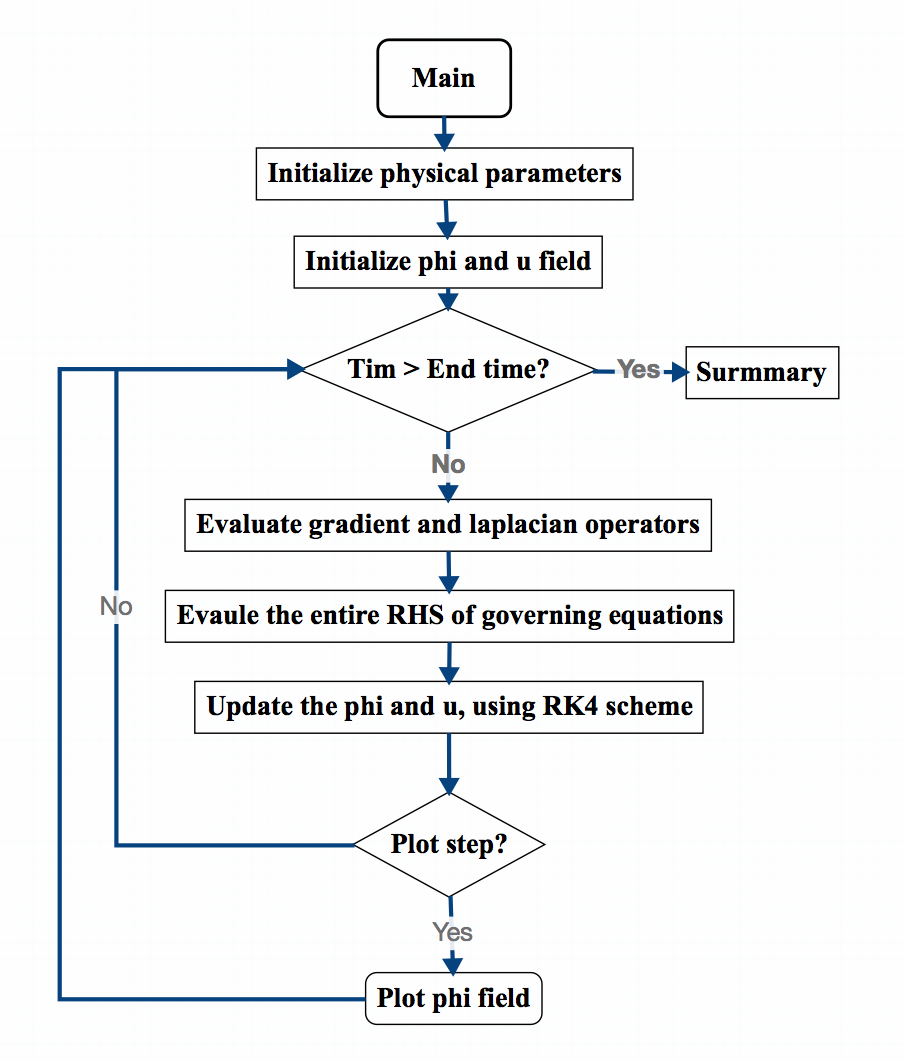
\includegraphics[width=1\textwidth]{flowchart_v_1} % Include the image placeholder.png
\caption{Figure caption.}
\end{center}
\end{figure}
\par \ 
\par 1. Initialize the modeling parameters including timestep dt, end time t, grid dh, domain size L, etc. 
\par 2. Initialize the $\phi$ and $u$ field.
\par 3. During one step, we calculate the gradient and laplacian by 
\par 4. Evaluate the orientation angle $\theta$, and then the $W$
\par 5. Evaluate RHS of $\phi$ euqation, update $\phi$ and then update $u$ by RK4
\par 6. Plot intermidiate time step contour of  $\phi$ and $u$
  
\section{Software Design}
The following existing classes will be directly utilized:
\begin{description}
\item[Point, Box, RectMDarray]
\item[RK4]
\item[VisitWriter, WriteRectMDArray]
\item[CH\_Timer]
\end{description}

\subsection{Analysis}
\begin{description}
\item[Output]
\item[Timer]
\end{description} 
	
\section{Optimization}
\section{Parameter Study} 
\section{Work Contribution} 

\end{document}